\documentclass[prl,aps,twocolumn,floatfix,amsmath,amssymb,superscriptaddress,tightenlines]{revtex4}
\usepackage{graphicx}% Include figure files
\usepackage{epstopdf}
%\usepackage{amsmath}
\usepackage{amsfonts}
\usepackage{bm}
%\bibliographystyle{prsty}
\begin{document}

\date{\today}
\title{Valence Bond and von Neumann Entanglement Entropy in Heisenberg Ladders}
\author{Ann B. Kallin}
\affiliation{Department of Physics and Astronomy, University of Waterloo, Ontario, N2L 3G1, Canada} 

\author{Iv\'an Gonz\'alez}
%TODO Decide on this!
%\affiliation{Fundaci\'on Centro Tecnol\'ogico de Supercomputaci\'on de Galicia (CESGA), Santiago de Compostela, Spain}
\affiliation{Centro de Supercomputaci\'on de Galicia, %(CESGA), 
Avda.~de~Vigo~s/n, E-15705 Santiago de Compostela, Spain}

\author{Matthew B. Hastings}
\affiliation{Microsoft Research, Station Q, CNSI Building, University of California, Santa Barbara, CA, 93106}

\author{Roger G. Melko}
\affiliation{Department of Physics and Astronomy, University of Waterloo, Ontario, N2L 3G1, Canada} 

\begin{abstract} We present a direct comparison of the recently-proposed
valence bond entanglement entropy and the von Neumann entanglement entropy on
spin-1/2 Heisenberg systems using quantum Monte Carlo and density-matrix
renormalization group simulations.  For one-dimensional spin chains we
show that the valence bond entropy can be either less or greater than the
von Neumann entropy, hence it cannot provide a bound on the latter.  On
ladder geometries we reproduce a multiplicative logarithmic correction
previously found in the area law for valence bond entropy in the
two-dimensional limit.  In this N\'eel state, the von Neumann entropy
obeys the area law without correction.

\end{abstract}
\maketitle

%\newpage

{\it Introduction.}-- Entanglement has arisen 
as a new paradigm for the study of correlations in condensed matter systems.  
Measurements
of entanglement between subregions, chiefly using entropic
quantities, have an advantage over traditional two-point correlation
functions in that they encode the total amount of information shared
between the subregions without the possibility of missing ``hidden''
correlations \cite{wolf}.  
Such correlations may occur in some quantum groundstates,  for example spin liquid states, 
where two-point correlation functions decay at large lengthscales, however a type of topological order can exist that is quantified in a ``topological entanglement
entropy''  \cite{ KP, LW}.
This and other entropic measures are typically discussed in the context of
the von Neumann (VN) entanglement entropy (EE), which for a system partitioned into
two regions A and B, quantifies the amount of entanglement of A with B as
\begin{equation} 
S^{\rm VN}_A = - {\rm Tr} [ \rho_A \ln \rho_A ]. \label{vNEE} 
\end{equation}
Here, the reduced density matrix $\rho_A = {\rm Tr}_B | \psi \rangle
\langle \psi |$ is obtained by tracing out the degrees of freedom
associated with the region B.

The properties of the VN EE are well-studied in the context of quantum information theory.
In interacting one dimensional (1D) quantum systems, exact analytical results are known from conformal
field theories (CFT); they show that, away from special critical points,
the VN EE scales as the size of the boundary between A and B.
This so-called {\it area law} \cite{Shredder} is also believed to hold in many
groundstates of two dimensional (2D) interacting quantum systems,
although few exact results are available \cite{ALreview}.  This has 
consequence in the
rapidly-advancing field of computational quantum-many body theory, where
it is known for example that groundstates of 1D Hamiltonians that satisfy an area law
can be accurately represented by Matrix Product States (MPS) \cite{MPS_DMRG}.
Tensor-network extension of MPS states are the basis
for a new promising class of numerical algorithms \cite{PEPS1,PEPS2} that may push our
abilities to simulate 2D quantum systems past that
allowed by quantum Monte Carlo (QMC), which is hampered by
the notorious fermionic sign problem.  However, tensor network states
are constructed to obey an area law; in order to be represented faithfully
by them, a given 2D quantum groundstate must have physical entanglement
properties which also obey the area law \cite{ALreview}

%However, it is believed that 2D
%states which lend themselves to accurate approximation by such methods
%must also obey an area law.

%\begin{figure} { 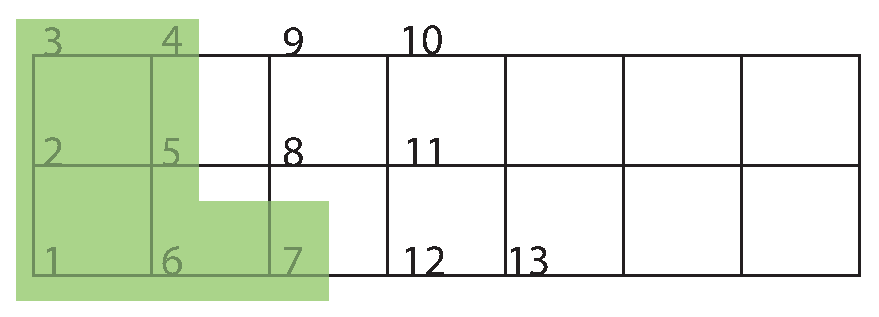
\includegraphics[width=2.4in]{ladder.eps}
%\caption{(color online) A three-leg ladder.  The site labels $x$ indicate
%the order in which DMRG sweeping takes place, which is also the index
%order by which entanglement entropy is measured.  The blue box labels
%sites in the region A, with $x=7$.  \label{ladder}}} \end{figure}

Unfortunately, entanglement is a quantity that is difficult to
measure in 2D systems.  This is due to the fact that QMC - currently the
only scalable method capable of unbiased 2D simulations - does not have
direct access to the groundstate wavefunction $| \psi \rangle$, required
in Eq.~\eqref{vNEE}.  In response to this, several authors \cite{Alet,
Chh} has recently introduced the concept of {\it valence bond} (VB)
entanglement entropy, defined for a  spin system as
\begin{equation} 
S^{\rm VB}_A = \ln(2) \cdot \mathcal{N}_A, \label{VBEE}
\end{equation} 
where $ \mathcal{N}_A$ is the number of spin singlets
${( |\uparrow \downarrow \rangle - | \downarrow \uparrow
\rangle)/\sqrt{2}}$ crossing the boundary between regions A and B.  Unlike
the VN EE, the VB EE can be accessed easily in the valence-bond basis
projector QMC method recently proposed by Sandvik \cite{Sandvik}.  As
demonstrated in Refs.~\cite{Alet,Chh}, the VB EE has many properties in
common with the VN EE, in particular the relationship $S_A = S_B$, and the
fact that $S^{VB}_A=0$ for regions ``un-entangled'' by valence bonds.
Further, a comparison of the scaling of the VB EE for (critical) 1D spin
1/2 Heisenberg chains shows good agreement with analytical results known
from CFT.  What is
particularly striking \cite{Alet,Chh} is that the VB EE in the
 2D isotropic Heisenberg model
displays a {\it multiplicative} logarithmic correction to the area law, a property
which would have negative consequences for the simulation of the 
N\'eel groundstate using tensor-network simulations.

%If this
%property were to be shared by the VN EE, it could have the consequence
%that the 2D Neel groundstate can not be approximated by a tensor-network,
%and is therefore not amenable to simulation techniques based on the MPS
%framework
 
In this paper, we compare the VB EE calculated by valence-bond QMC to the
VN EE accessible through density-matrix renormalization group
(DMRG) simulations of the Heisenberg model on $N$-leg ladders.    For $N=1$, the CFT central charge calculated  by scaling the
VN EE shows excellent agreement to $c=1$, whereas the VB EE appears to converge
to $c<1$.
For $N>1$, the VB EE is systematically greater than the VN EE,
a trend which grows rapidly with $N$. An
examination of entanglement defined by bisecting multi-leg ladders
shows a logarithmic correction for the VB EE, $S^{VB}_A /N = N \ln
N$ (in agreement with Refs.~\cite{Alet,Chh}), however for data up to
$N=7$, the VN EE convincingly shows a scaling of
$S^{VB}_A /N = N$, thus obeying the area law.

{\it Model and Methods.}-- We consider the spin 1/2 Heisenberg
Hamiltonian, given by  
$H =  \sum_{\langle i j \rangle}
{\mathbf S}_i \cdot {\mathbf S}_j \label{ham}$, 
where the sum
is over nearest-neighbor sites.  Geometries studied are 1D chains, and
multi-leg ladders with length $L$ and number of legs $N$.  
%Many properties of this model on open-boundary ladders with $n$ legs has
%been exhaustively studied.  Of importance, it is known that a spin gap
%exists for even-$n$ ladders in the limit of $L\rightarrow \infty$,
%whereas odd-$n$ ladders behave somewhat more like quasi-1D  systems with
%spin $n/2$ and, from Haldane's conjecture, are therefore gapless.  
We employ two complementary numerical techniques in our study of EE on
ladder geometries, namely the valence-bond basis QMC and DMRG, both of
which give {\it unbiased} approximations to the ground state of the
Hamiltonian at zero temperature, and results from both of which can be
compared directly to one another.  The VN EE is naturally accessible
through the DRMG ``sweeping'' algorithm~\cite{White92, Scholl05}.  At each
step of the algorithm, the wavefunction of the system is approximated by
keeping only the states with largest coefficients in the Schmidt's
decomposition for subregions A and B. To find the basis entering the
Schmidt's decomposition for subregion A, the reduced density matrix
$\rho_A$ is calculated and diagonalized, thus allowing easy calculation
of Eq.~\eqref{vNEE}. The truncation of the basis implies that only an upper
bound for $S^{VN}_{A}$ is calculated, so care must be taken to ensure
that enough of the eigenvalue spectrum is included to converge the VN EE
to sufficient accuracy; typically the number of states required is larger
than that needed to converge the energy alone.

The VB EE \cite{Alet,Chh} can be calculated using the valence-bond basis
QMC proposed by Sandvik \cite{Sandvik}.  The valence-bond basis QMC
algorithm that we use is the simple single-projector method, with lattice
geometries constructed to match those given by the DMRG algorithm.  The
ground state of the system is projected out by repeated application of a
list of bond operators on nearest neighbor sites of the ladder.  A number
of bond operators ($r$) are changed each step and the change is accepted
with a probability depending on the number of nearest neighbor bonds in
the resulting valence bond states. Measured quantities such as energy or
VB EE are then calculated by a weighted average over all the valence bond
states obtained by this procedure.

\begin{figure} {
%
\includegraphics[width=3.2in]{fig1_inset.eps}

\includegraphics[width=3.3in]{4-panelFIG1.eps} \caption{(color online) VB
and VN entanglement entropies for 1D Heisenberg model with PBC (left
panels), and OBC (right panels). Upper panels show the entropies as a
function of the conformal distance $x'$ for 100-site chains (see text).
Lower plots show the values for the central charge $c$, obtained by
fitting the numerical data to the CFT result, for several chain lengths.
For PBC (left panel), $c$ is plotted as a function of inverse system size.
For OBC (right panel), boundary effects make the fits depend on the number
of sites included in the fit, $z$. To bypass these effects we plot $c$ as
a function $z$ for each $L$. Here, $z$ is systematically decreased by
removing points from the {\it outside} ends of the open-boundary chain.
$c$ is illustrated for the VN EE (closed symbols) and the VB EE (open
symbols) for system sizes $L=64$ (circles), $L=100$ (squares), $L=128$
(diamonds), and $L=200$ (triangles) \label{1D}}} \end{figure}

{\it One-dimensional chain.}-- We consider first the case of 1D Heisenberg
chains. We employ both open (OBC) and periodic (PBC) boundary conditions
with our DMRG and QMC simulations,
% in order to study the VN and VB entanglement entropies
noting that in the DMRG, PBCs typically have poorer convergence properties than OBCs
and more states must be kept in each truncation.
% It's better now. We can delete this comment, and clean this up.
% I MODIFIED THIS A BIT ABOVE: CHECK IT OUT GONZ
% 
%TODO
% I will delete this sentence between brakets if needed: this is well
% known and does not bring much to the paper discussion
The DMRG algorithm requires each subregion A and B to be topologically
connected, so in 1D the bipartition is defined by a site index $x$ with
sites within the interval $[1,x]$ ($[x+1,L]$) belonging to subregion $A$
($B$), $L$ being the length of the chain. 
%I ADDED THE BELOW ALSO
From the remainder of this paper, we label the EE $S_A$ by its site index, $S(x)$.
%
We stress that the QMC and DMRG
results are on the same geometry and Hamiltonian, and reproduce the same
ground state energies; all the figures in this paper can be considered as
exact comparisons between the VB and VN EE. 

The 1D Heisenberg model is known to be critical and therefore can be
mapped to a 2D classical Hamiltonian at its critical point, which in turn
can be described within CFT in the limit $L\to\infty$.  To address
finite-length chains one can use the conformal mappings $x\to x'=L/\pi
\sin(\pi x / L)$ for PBC, and $x\to x'=2L/\pi \sin(\pi x / L)$ for OBC. VN
EE calculations within CFT~\cite{Cardy, Huanq2006} obey $S^{VN}(x)= c/3
\ln(x') + S_1$ in the PBC case, and $S^{VN}(x)= c/6 \ln(x') +
\ln(g)+S_1/2$ in the OBC case, where $c$ is the central charge of the CFT,
$S_1$ is a model-dependent constant, and $g$ is Ludwig and Affleck's
universal boundary term~\cite{AffleckAndLudwig}.

Figure~\ref{1D} illustrates simulation results in both cases, the left
(right) panels corresponding to PBC (OBC). In Refs.~\cite{Alet, Chh}, VB
EE calculated from QMC was compared to the CFT result, and a good fit to a
central charge of $c=1$ was found for both cases.  In Fig.~\ref{1D} we
compare this result to the VN EE calculated from the DMRG.  For PBC both
the VN and VB entropies are seen to fit well to the CFT result, although
the VN EE is greater than the VB EE. The regression fit shows very good
convergence with the CFT central charge prediction for the VN EE, while
the VB EE fit yields a lower value than predicted.  
%TODO {\it (Should I include this?) It is possible the VB EE data is not
%sufficiently converged which would could give results below the CFT
%predicted value, however data from Refs.~\cite{Alet,Chh} bears similar
%results. }

For OBC both the VN and VB EE split into two branches, the upper (lower)
corresponding to an odd (even) number of lattice sites in $A$.  This
reflects a well-known ``dimerization'' effect induced by OBC~\cite{Ian1}.
Notice that contrary to the PBC case, the VN EE is now \textit{smaller}
than the VB EE. A regression fit of the lower branch to the form $c/6 \ln
{x'}$ (inset) shows excellent convergence of the VN EE to the central
charge predicted by CFT, $c=1$, once finite-size effects and the proximity
of the data to the open boundaries are taken into account.  In contrast,
the VB EE fit deviates significantly from the CFT result for larger system
sizes, give $c>1$ when all or most data is included in the fit, and $c<1$
as data is systematically excluded from the fit (data closest to the open
boundary is removed first).

{\it Multi-leg ladders.}-- Moving away from the 1D chain, one can add
``legs'' to the lattice in a systematic way. In this case the sum over
nearest neighbors is extended to neighbors along rungs as well as along
legs.  As it was noted before, DMRG imposes contraints to the subregion
geometry. In multi-leg ladders we choose to move in a 1D path that visits
first bonds sitting in rungs rather than bonds sitting in legs (see
Fig.~\ref{ladder}). 
%One of such paths is illustrated in the bottom left inset of
%Fig.~\ref{ladder}.
DMRG computational demands increase dramatically with the number of legs,
so in this paper we restrict ourselves to ladders up to $N=6$ legs with
OBC. VB QMC lacks of this limitation and we are able to go up to $N=24$. 
%TODO Ann: Could you confirm this 24 for QMC ?.

\begin{figure} { 
\includegraphics[width=3in]{FIG2.eps} \caption{(color
online) VB and VN entanglement entropies for 4-leg ladder (upper panel)
and 3-leg ladder (lower panel) systems with OBC and 100 sites per leg.
(Upper panel) Left inset shows the site indexing used for multi-leg
ladders. The shadowed area shows the bipartition for $x=9$. Right inset
shows details of the central region of the ladder and the periodic
structure on $S(x)$.  For even-leg ladders the period is $N$. (Lower
panel) Left inset shows $S(x)$ as a function of the conformal distance,
$x'$.  Right inset shows details of the central region of the ladder and
the periodic structure on $S(x)$. For odd-leg ladders the period is $2N$.
\label{ladder}}} \end{figure}

\begin{figure} {
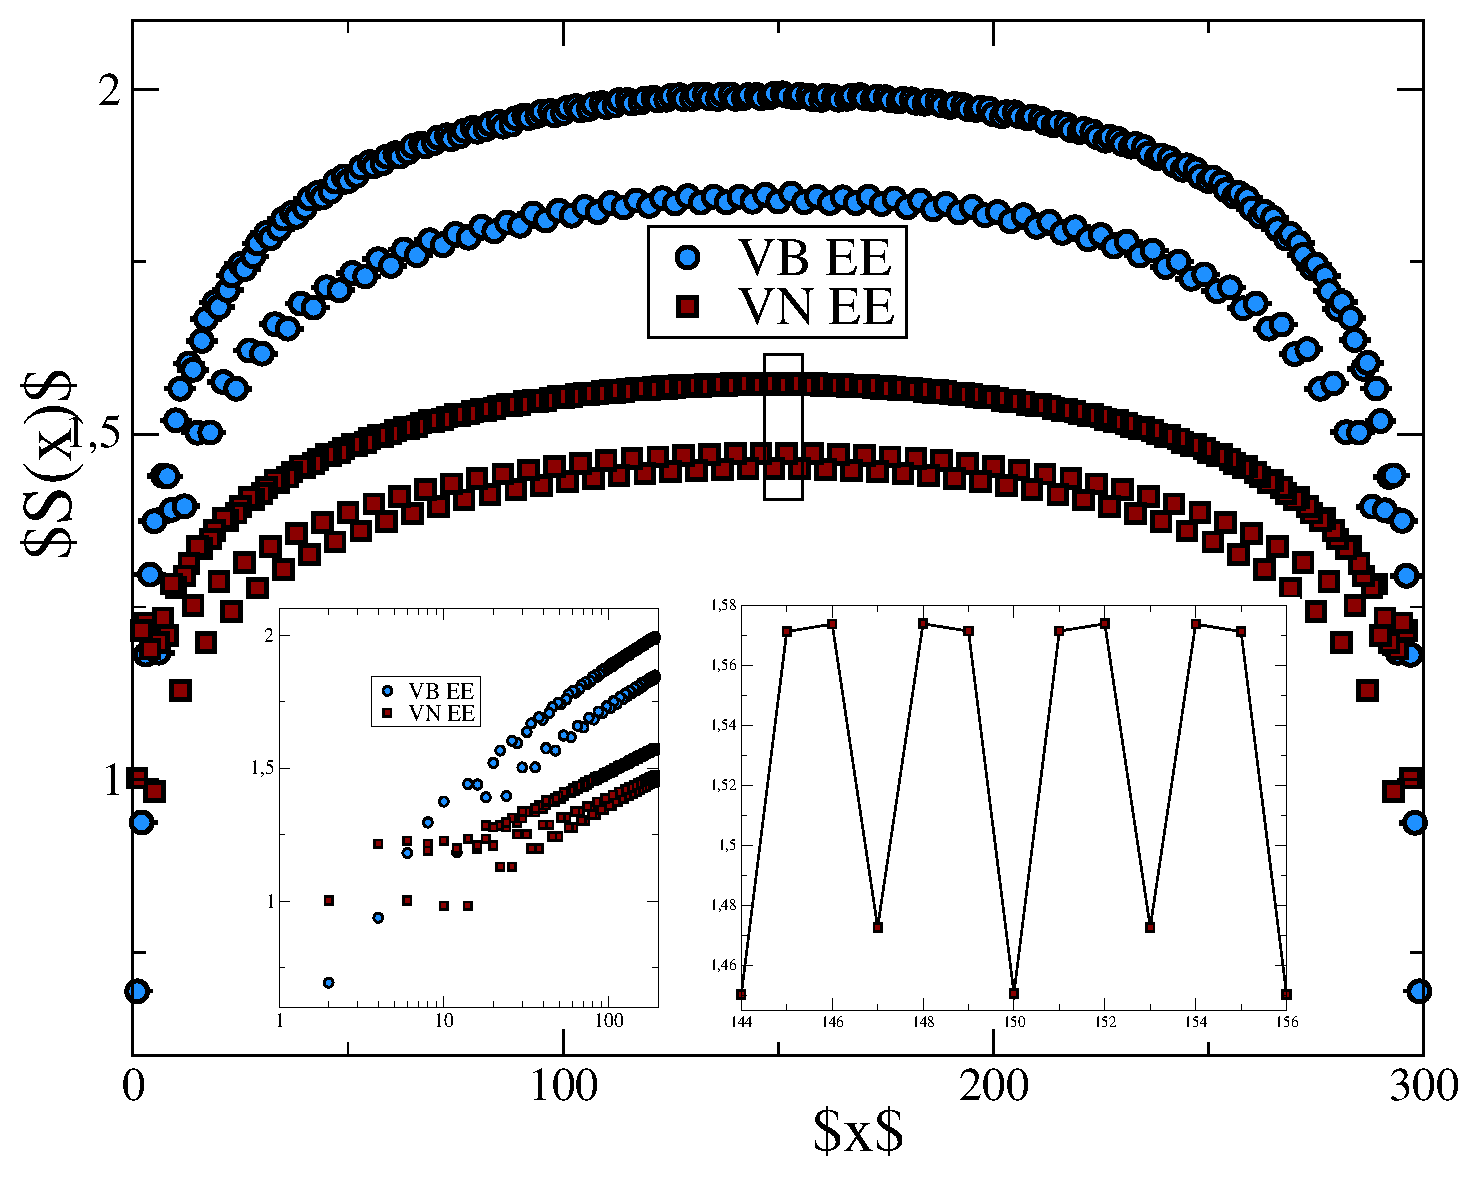
\includegraphics[width=3in]{figure3/3-leg-ladder/fig3_final.eps} \caption{(color
online)  \label{odd-ladder}}} \end{figure}

$S(x)$ shows a different behavior depending on $N$ being even or odd.
Even-leg ladders are known to have a spin-gap~\cite{White1994}, 
%which decreases with $N$, and therefore local operators in sites
%separated by distances larger than the corresponding correlation length
%are expected to be un-correlated.
and therefore only sites at distances from the boundary between A and B
smaller than the correlation length $\xi$ are expected to contribute to
the entanglement, yielding $S(x\gtrsim \xi)=const.$ Figure~\ref{ladder}
shows the VB and VN entanglement entropies calculated for the 4-leg
ladder. As expected for large subregion sizes the EE are constant with
$x$. As happens with the 1D chain, the VB EE is larger than the VN EE, and
as will discused below, this difference increases with increasing $N$. It
can be seen that $S(x)$ develops a periodic structure with period $N$. A
qualitative explanation based on a RVB picture is the following. An
even-leg ladder can be covered by singlets formed by spins on the same
rung of the ladder. 
%TODO this is shitty and too long.
Although the energy of this VB state is the same as any other it has more
possibilities to resonate, e.~g. by forming plaquettes.  Long-range bonds
connecting sites in distant rungs create a ``stagered'' regions which can
not resonate and therefore give a RBV state with higher
energy~\cite{White1994}.  Within this picture, one expects higher EE
values when the boundary between A and B cuts a bond sitting in a rung,
$x\equiv0 \mod{N}$, than when cuts only bonds in legs, $x\equiv0 \mod{N}$.
Within the same rung, sites at the ends will tend to form singlets with
its only neighbor in the rung and EE will be larger for $(x\div N) \equiv
1 \mod{2}$, than for $(x\div N) \equiv 0 \mod{2}$.

Odd-leg ladders are gapless, and therefore all the sites within subregions
A and B are expected to contribute to the entanglement and similarly to
the 1D case, $S(x)$ is expected to have a maximum at $x=L/2$. 
Figure~\ref{ladder} shows the VB and VN entanglement entropies calculated
for the 5-leg ladder. Again VB EE os larger than VN EE. It can be seen
that $S(x)$ develops a periodic structure which in this case has period
$2N$. Following the afore-mentioned qualitative RVB picture, one can see
that as the odd-leg ladders can not be covered only by singlets sitting in
rungs, long-range VB are not penalized. 

{\it Area law in multi-leg ladders.}--  
Given the ground state of a
quantum many-body system in 2D, the question of whether the entanglement
entropy fulfills and "area" (boundary) law is in general a difficult one
to answer.  
%However from a simulation perspective this question is of
%utmost importance, since tensor-network generalization of MPS techniques,
%such as PEPS, produce states that satisfy the area law by construction.
%Thus in order to simulate, for example, the N\'eel groundstate of the 2D
%Heisenberg model accurately with such methods depends critically on
%whether or not the entanglement entropy of the N\'eel state obeys an area
%law.  
Using VB EE, Refs.~\cite{Alet,Chh} examined this issue for the 2D Heisenberg model and found
multiplicative logarithmic corrections to the area law in the N\'eel
state, which was attributed to gapless Goldstone modes and
algebraically decaying correlations.  
We can address this question further using our data for the VB and VN EE discussed 
in the above section on multi-leg ladders.  That is, we chose a lattice
geometry such that subregion A is rectangular, cutting a multi-leg ladder
cleanly across a rung, such that the ``area'' separating region A and B is
equivalent to the number of legs in the ladder $N$.  We chose this area A
to contain contain $2N^2$ sites ...{\bf Matt: do we want to spell out the
argument involving the sum over quasi-1D modes?  I think we will have
room}.

Figure~\ref{zigzag} illustrates the simulation results for $N$-leg ladders.
Plotting $S_A/N$ versus $N$ on a log scale, one sees that we reproduce the
multiplicative logarithmic correction to the VB area-law, in agreement
with Refs.~\cite{Alet,Chh}.  However, the linear slope is not present in
the plot of the VN EE data from the DMRG, which convincingly approaches a
constant for large $N$.  Clearly, the VN EE suggests that the area law is
indeed obeyed in the N\'eel groundstate, leading one to conclude that the
multiplicative logarithmic correction is an artifact of the VB EE.

%Despite the importance of adherence to the area law in tensor-network
%generalization of MPS techniques, it is still not yet known whether the
%2D isotropic Heisenberg ground state does obey the area law.  The results
%from Refs.~\cite{Alet,Chh} for the VB EE in 2D indicate a multiplicative
%logarithmic corrections to the area law.  We find it necessary to address
%whether the same logarithmic correction exists in the VN EE.
%Fig.~\ref{zigzag} shows the VB EE and VN EE for ladders with N legs.  The
%lattice geometry is chosen such that subregion A contains $2N^2$ sites
%and is always rectangular.  It is clear that Fig.~\ref{zigzag} shows a
%logarithmic correction to the area law for VB EE, in agreement with
%Refs.~\cite{Alet,Chh}.  However, in the case of the VN EE, the data
%approaches a constant value and shows no correction to the area law.

\begin{figure} { 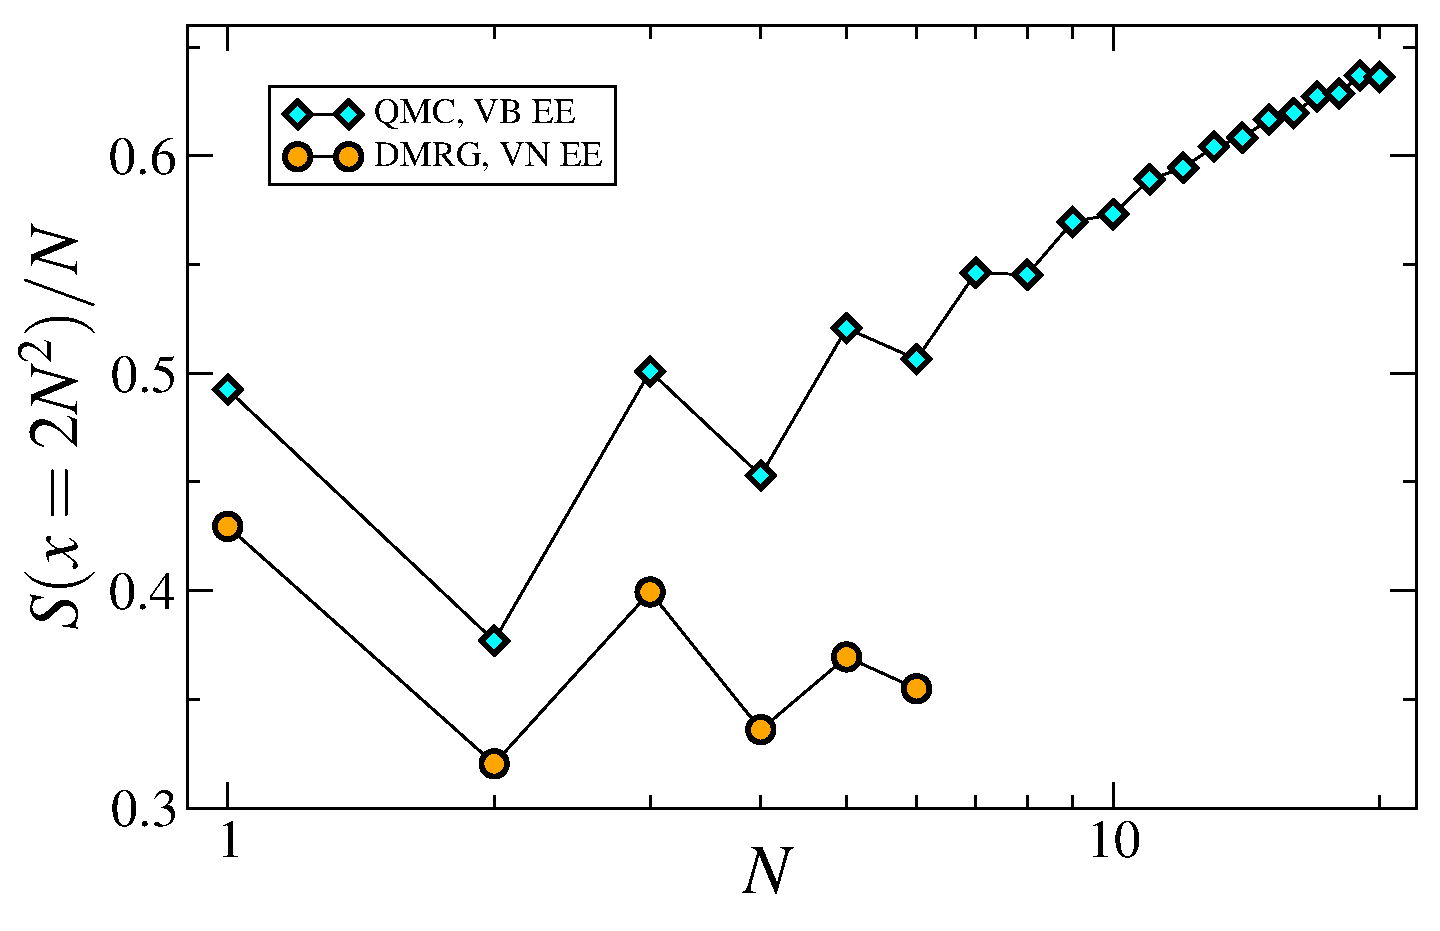
\includegraphics[width=3in]{fig4.eps} \caption{(color
online) VB and VN entanglement entropies (taken such that the region A
includes $2N^2$ sites) normalized by N, the number of legs.  All ladders
have 100 sites per leg.  \label{zigzag}}} \end{figure}

{\it Discussion.}-- In this paper, we have compared scaling properties of
the valence bond (VB) entanglement entropy (EE) defined in
Refs.~\cite{Alet,Chh} to the von Neumann (VN) entanglement entropy in the
spin 1/2 Heisenberg model on 1D and multi-leg ladder geometries.  Both
entropy measurements were evaluated using large-scale numerical
simulations; the VN EE with DMRG, which is restricted to 1D or seven-leg
and less open boundary ladders; and the VB EE with valence-bond basis QMC,
which is avaliable for any lattice dimension or geometry. In 1D, we find
that the VB EE mimics the behavior of the VN EE closely, although using
the definition of Eq.~\eqref{VBEE}, is less than the VN EE for periodic
chains, and greater than the VN EE for open chains. In addition, fits to
1D conformal field theory, which are excellent for the VN EE calculated
via DMRG, appear to deviate significantly for the VB EE in the large
chain-size limit, approaching some $c<1$ for both boundary conditions
examined here.

On multi-leg ladder systems with open boundaries, the VB EE is
systematically greater than the VN EE, a discrepancy which grows as the
number of legs in increased.  Defining the boundary between the two
entangled regions as being bipartitioned by a cut across all legs, we can
evaluate an ``area law'' in the ladder geometries.  The VN EE measured by
DMRG adheres to the area law in the large-leg limit, whereas the VB EE
measured by QMC reproduces a multiplicative log correction found in
Refs.~\cite{Alet,Chh} for the N\'eel groundstate of the 2D Heisenberg
model.

This work has elucidated the relationship between the VB and VN EE.
Although clearly a good measurement of entanglement readily accessible to
numerical simulations in 2D and higher, the VB EE does not provide a bound
on the VN EE, unlike other entropic measures such as Renyi entropies.
Other properties of the VN EE, such as its adherence to an area law, are
reproduced in the groundstates of some gapped systems \cite{Alet,Chh},
however in the case of the N\'eel groundstate of the 2D Heisenberg model,
unphysical multiplicative logarithmic corrections appear in the VB EE,
which are not caused by gapless excitations or algebraically decaying
correlations, but simply by the valence-bond length distribution ({\bf we
need to justify this in the text}).  The presence of this correction must
be taken into account in proposals to use the VB EE for such important
future tasks such as characterizing topological phases using entanglement
entropy, or studying universality at quantum phase transitions.

{\it Acknowledgements.}-- The authors thank I.~Affleck, J.~Berlinsky,
A.~Del~Maestro, A.~Feiguin, L.~Hormozi, and E.~Sorensen for useful
discussions.  This work was made possible by the computing facilities of
SHARCNET and CESGA.  Support for this work was provided by NSERC of
Canada.

\bibliography{VB_biblio}

\end{document}
